
\chapter{基于 Libfvphg 库的三维非结构网格算例}
\label{chap:libfvphg-improve}

\section{Libfvphg 库简介}
\label{sec:phg--libfvphg}

本章的主要工作是基于滕飞博士的 Libfvphg \cite{tengfei2010} 库完成
的. Libfvphg 是对并行自适应有限元平台 PHG 相关功能的进一步封
装, 以 \Cpp 函数库的形式为三维非结构网格有限体积解法器的实现提供了
一个整体框架. 本章的主要工作是在 Libfvphg 的基础上实现了三
维 MUSCL 类型有限体积法, 使用典型的算例进行验证, 并对其并行效率进
行了测试. 下面首先简要介绍 Libfvphg 的基本工作原理.

Libfvphg 框架下的计算主要可以分为如下几个步骤, 以计算进行到第 $n$
时间步为例,
\begin{description}
\item[第一步] 依据 CFL 条件, 利用当前时间层的单元平均值计算时间推
  进步长 $\Delta t ^{n}$. 首先计算每个单元上所允许的最大时间步长,
  \begin{equation}
    \label{eq:cfl-condition}
    \Delta t^{n}_{j} =  \frac{\vert T_{j}
      \vert}{\alpha_{j} ~ \sum_{k=1}^{4}\vert f_{j,k} \vert}
  \end{equation}
  其中 $f_{j,k}$ 为单元 $T_{j}$ 的第 $k$ 个面. $\alpha_{j}$ 为局
  部特征值的最大值,
  \begin{equation}
    \label{eq:local-maximum-eigen}
    \alpha_{j} = \max (\lambda_{j}^{max}, \max_{k} \lambda_{j,k}^{(max)}).
  \end{equation}
  则该时间层的推进步长应取其中的最小值,
  \begin{equation}
    \label{eq:minimal-time-step}
    \Delta t^{n} = \kappa_{{cfl}} \min_{T_{j} \in
      \mathcal{T}} \Delta t^{n}_{j}
  \end{equation}
  其中 $\kappa_{{cfl}}$ 是人为参数, 用于控制时间步长的大小.
\item[第二步] 利用当前时间层的网格平均值 $\left\{ \bar{u}^{n}_{j}
  \right\}_{j}$ 重构得到单元边界上 Gauss 积分点 $\left\{ x_{T,
      f,l} \right\}_{T \in \mathcal{T},f \in \partial T,l}$ 的高阶
  重构值. 文献 \cite{tengfei2010} 采用的是 Cockburn 、Shu 在文
  献\cite{Cockburn1998} 中二维三角形网格间断有限元方法设计的线性重
  构策略. 但是在实际计算中我们发现该策略数值稳定性较差, 在处理变化
  较为剧烈的 Euler 方程算例时会出现负压强的状况. 我们实现了
  Barth-Jespersen 限制策略, 获得了较好的稳定性.
\item[第三步] 利用重构值计算积分点处的数值通
  量 $h(\tilde{u}^{int},\tilde{u}^{ext},{\bf{n}})$. 计算中采用的
  是 Local
  Lax-Friedrichs 通量
  (\ref{eq:local-lax-friedrichs-flux}).
\item[第四步] 使用 SSP Runge-Kutta 方法 (\ref{eq:second-order-rk}
  - \ref{eq:3rd-rk}) 进行时间推进. 在 Runge-Kutta 方法的每一个分
  步骤, 都需要执行一次上面的第二第三步, 以确定空间离散 $\mathcal{L}$.
\item[第五步] 依据误差指示子进行后验误差估计, 用特定的自适应策略对
  网格进行放粗或加密, 实现 h-自适应计算.
\end{description}

\section{测试算例}
\label{sec:numerical-parallel}

本节的测试算例都是针对三维的 Euler 方程. 其控制方程为,
\begin{equation}
  \label{eq:3d-euler-eq}
  {\bf{U}}_{t} + {\bf{F}}({\bf{U}})_{x} + {\bf{G}}({\bf{U}})_{y}
  + {\bf{G}}({\bf{U}})_{y} = 0,
\end{equation}
其中,
\begin{equation}
  \label{eq:3d-euler-eq-notation}
  \left.
    \begin{aligned}
      &{\bf{U}} = \left[
        \begin{array}{c}
          \rho\\
          \rho u\\
          \rho v\\
          \rho w\\
          E
        \end{array}
      \right], \quad
      {\bf{F}}({\bf{U}}) = \left[
        \begin{array}{c}
          \rho u\\
          \rho u^{2} + p\\
          \rho uv \\
          \rho uw \\
          (E+p) u
        \end{array}
      \right],\\
      &{\bf{G}}({\bf{U}}) = \left[
        \begin{array}{c}
          \rho v\\
          \rho u v\\
          \rho v^{2} + p\\
          \rho v w\\
          v (E + p)
        \end{array}
      \right], \quad
      {\bf{H}}({\bf{U}}) = \left[
        \begin{array}{c}
          \rho w\\
          \rho u w\\
          \rho v w\\
          \rho w^{2} + p\\
          w (E + p)
        \end{array}
      \right].
    \end{aligned}
  \right\}
\end{equation}

在测试算例中使用的非结构网格均由非结构网格工具 GMSH
\cite{Geuzaine2009} 所生成. 另外, 所有大规模并行算例都是在科学与
工程计算国家重点实验室的 LSSC-\Rmnum{3} 集群上完成.

\subsection{三维激波管问题}
\label{sec:sod-shock-tube-test-case}

激波管问题的初始工况如图 (\ref{fig:sock-tube-illustration}) 所示.
管道内部由一个厚度可以忽略的隔膜将其分成左右两部分, 在 $t = 0$ 时
刻突然将隔膜移开. 研究在此之后管道内气体的演化问题就是激波管问
题. 在理想气体条件下忽略粘性的影响, 激波管问题就是一维的 Riemann
问题. 其精确解可以由 Riemann 求解器得到.

\begin{figure}[htbp]
  \centering
  \newcommand\MYheight{1}
\newcommand\MYwidth{1.5}

\begin{tikzpicture}[scale=2.2]
 
\coordinate (LM) at (0,0);
\coordinate (UM) at (0,\MYheight);
\coordinate (UL) at (-\MYwidth,\MYheight);
\coordinate (LL) at (-\MYwidth,0);
\coordinate (UR) at (\MYwidth,\MYheight);
\coordinate (LR) at (\MYwidth,0);
\coordinate (CL) at (- 0.5 * \MYwidth, 0.5 * \MYheight);
\coordinate (CR) at (0.5 * \MYwidth, 0.5 * \MYheight);

 \draw[line width=1.0pt](LL) -- (LR);
 \draw[line width=1.0pt](UL) -- (UR);
 \draw[line width=1.0pt](LM) -- (UM);

\draw (CL) node {\scriptsize{$\rho_L, u_L, p_L$}};
\draw (CR) node {\scriptsize{$\rho_R, u_R, p_R$}};

\end{tikzpicture}
  \caption{Riemann 问题示意图}
  \label{fig:sock-tube-illustration}
\end{figure}

为表述方便, 规定 $x$ 方向为激波管的轴线方向. Riemann 问题的初始条
件可以表示为,
\begin{equation}
  \label{eq:shock-tube-initial-condition}
  {\bf{U}}|_{t=0} = \left\{
    \begin{aligned}
      & {\bf{U}}_{L} & \quad & \mbox{if} ~ x\le 0,\\
      & {\bf{U}}_{R} & \quad & \mbox{if} ~ x > 0.
    \end{aligned}
  \right.
\end{equation}
考虑如下的 Sod 问题 \cite{Toro2009},
\begin{equation}
  \label{eq:sod-initial-condition}
  {\bf{U}}_{L} := \left[
    \begin{array}{c}
      \rho_{L}\\
      u_{L}\\
      v_{L}\\
      w_{L}\\
      p_{L}
    \end{array}
  \right] = \left[
    \begin{array}{c}
      1\\
      0\\
      0\\
      0\\
      1
    \end{array}
  \right], \quad
  {\bf{U}}_{R} := \left[
    \begin{array}{c}
      \rho_{R}\\
      u_{R}\\
      v_{R}\\
      w_{R}\\
      p_{R}
    \end{array}
  \right] = \left[
    \begin{array}{c}
      0.125\\
      0\\
      0\\
      0\\
      0.1
    \end{array}
  \right].
\end{equation}
在该问题中, 左右两侧均无初始速度. 左侧为高密度高压区域, 薄膜移开之
后会产生左 ``侧稀疏波 -- 接触间断 -- 右侧激波'' 的波结构. 注意
到 (\ref{eq:sod-initial-condition}) 式是以原始变量的方式给出左右两
侧状态, 需要通过下面的热力学关系转换为守恒形式,
\begin{equation}
  \label{eq:primitive-to-conservative}
  E_{K} = \rho_{K} \left( e_{K} + \frac{1}{2} (u_{K}^{2} +
    v_{K}^{2} + w_{K}^{2}) \right), \quad e_{K} =
  \frac{p_{K}}{\rho_{K}(\gamma - 1)}.
\end{equation}

在该测试算例中, 以半径 $r= 0.1$ 长度 $l = 1.0$ 三维圆柱体作为计算
区域. 计算区域的中心位于坐标原点处. 使用 GMSH 以 $\mbox{lc} =
0.01$ 为特征尺度生成该计算区域的非结构网格. 这意味着在 $x$ 轴方向
平均分布有 100 个单元, 在 $r$ 方向平均分布有 10 个单元左右.  最终
生成的网格如图 (\ref{fig:3d-shock-tube-mesh}) 所示. 单元总数
为 135989.
\begin{figure}[htbp]
  \centering
  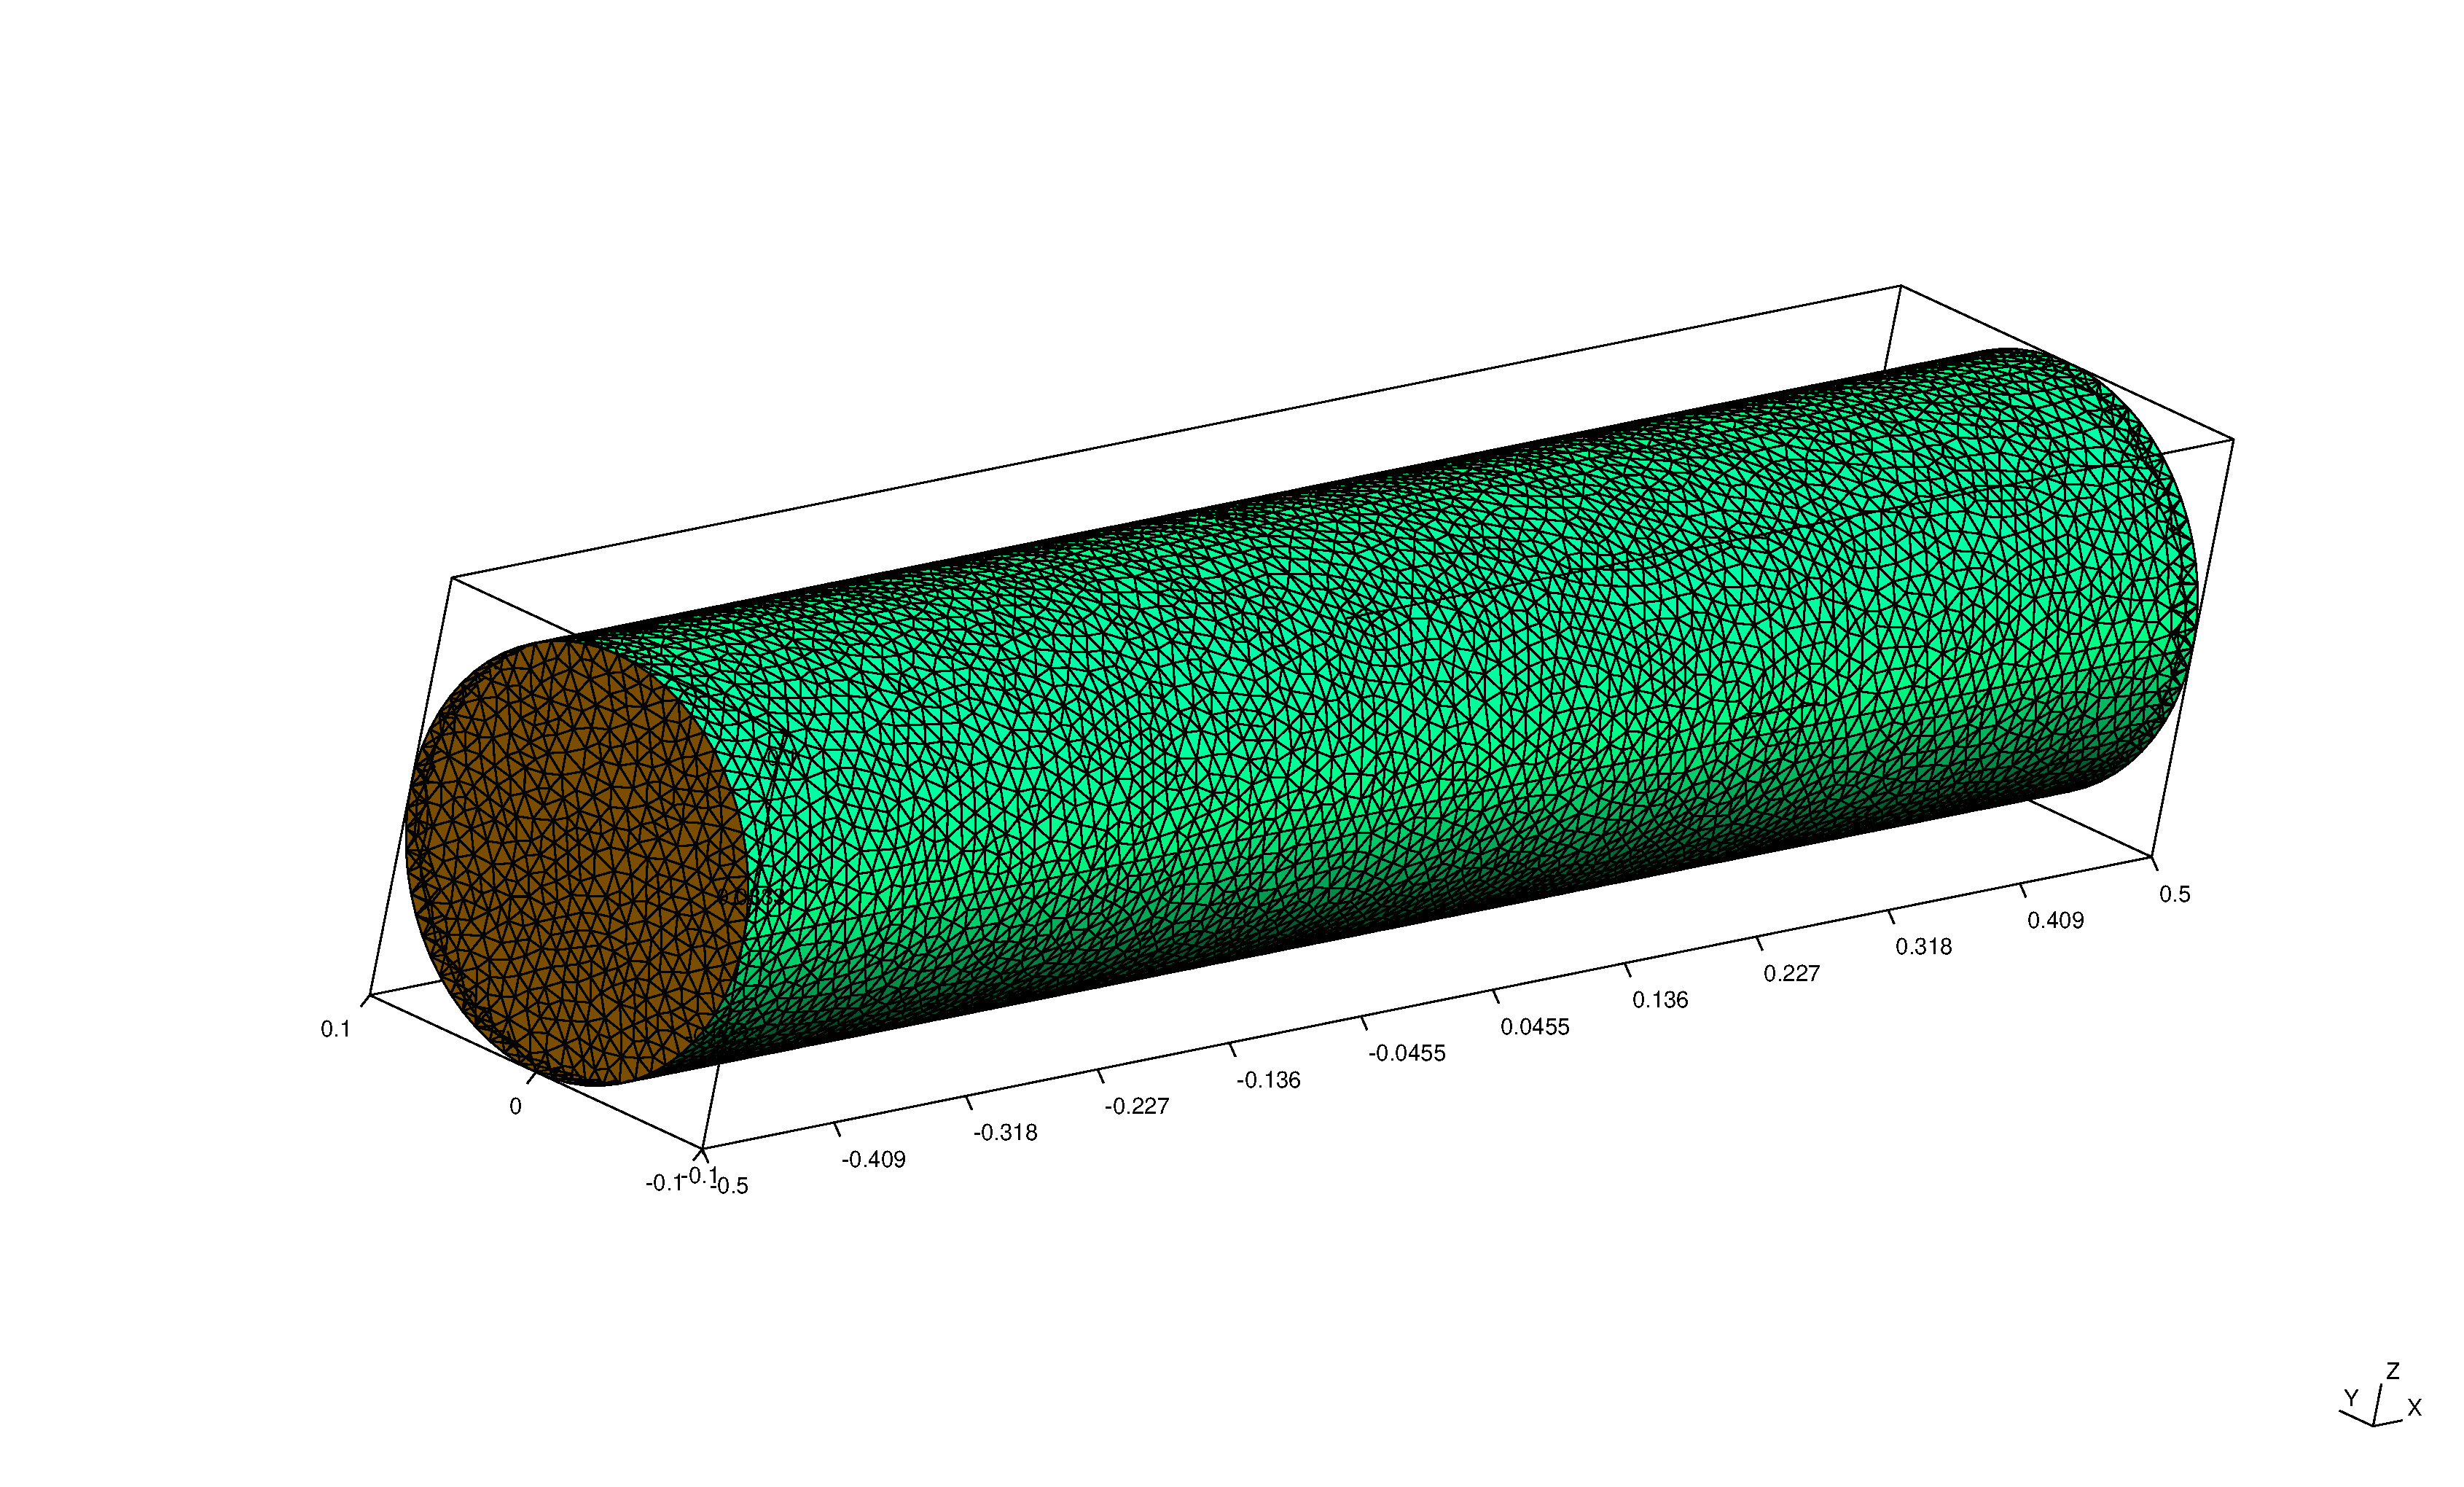
\includegraphics[scale=0.22]{./Pho/Chp4/shock_tube_mesh_fine.pdf}
  \caption{三维激波管问题所用网格}
  \label{fig:3d-shock-tube-mesh}
\end{figure}
关于边界条件, 激波管内壁采用固壁边界条件, 左右两端使用对称边界条
件. 计算终止时间为 $t_{end} = 0.2$. 计算结果如
图 (\ref{fig:sod-test-case-result}) 所示. 从计算结果可以看出, 三维
工况下的计算结果与一维精确 Riemann 求解器得到的结果基本吻合.
Barth-Jespersen 限制器作用下的二阶重构相比常值重构有一定的精度提
升, 但是仍然有很大的数值耗散, 没有体现出二阶方法在精度方面的优势.
\begin{figure}[htbp]
  \centering
  \includegraphics[scale=1.2]{./Pho/Chp4/shock_tube_sod_multiplot.pdf}
  \caption{三维激波管问题, Sod's case 计算结果}
  \label{fig:sod-test-case-result}
\end{figure}

\subsection{三维球对称爆炸问题}
\label{sec:3d-explosion-test-case}

Euler 方程三维球对称问题可以用带源项的一维方程进行描述, 此时所有
的变量都只依赖于时间 $t$ 及到对称中心的距离 $r$.
\begin{equation}
  \label{eq:3d-spherical-symmetry-euler}
  {\bf{U}}_{t} + {\bf{F}}({\bf{U}})_{r} = {\bf{S}} ({\bf{U}}),
\end{equation}
其中,
\begin{equation}
  \label{eq:3d-spherical-symmetry-euler-notation}
  {\bf{U}} = \left[
    \begin{array}{c}
      \rho \\
      \rho u_{r}\\
      E
    \end{array}
  \right], \quad
  {\bf{F}} = \left[
    \begin{array}{c}
      \rho u_{r}\\
      \rho u_{r}^{2} + p\\
      u_{r} (E + p)
    \end{array}
  \right], \quad
  {\bf{S}} = - \frac{\alpha}{r} \left[
    \begin{array}{c}
      \rho u_{r}\\
      \rho u_{r}^{2} \\
      u_{r} (E + p)
    \end{array}
  \right]
\end{equation}
其中 $u_{r}$ 表示流体沿径向的速度. 参数 $\alpha$ 表征了问题的维度,
$\alpha = 0$ 时方
程
(\ref{eq:3d-spherical-symmetry-euler}-\ref{eq:3d-spherical-symmetry-euler-notation})
退化为一维的 Euler 方程, $\alpha = 1$ 时则描述了二维的柱对称问题,
$\alpha = 2$ 则对应了三维的球对称问题.
(\ref{eq:3d-spherical-symmetry-euler-notation}) 式中
的 ${\bf{S}}$项称为几何源项. 在数值算例中, 可以使用相对成熟的一维
高精度求解器进行求解. 在下面的数值算例中, 我们用这种计算策略得到对
高维情形的参考解.

球对称爆炸问题中, 初始状态为计算区域的中间 $r < R_{c}$ 部分为高压高密
度核心, 外围区域则为低压低密度区域. 因此该问题可以视为一维的 Riemann
问题在高维的推广. 在下面的数值计算中, 设定计算区域为半径 $R =
1.0$ 的球体. 核心部分区域半径 $R_{c} = 0.4$.

初值的设定仿照 Sod 激波管问题,
\begin{equation}
  \label{eq:3d-spherical-symmetry-euler-initial}
  {\bf{U}}|_{t = 0} = \left\{
    \begin{aligned}
      &{\bf{U}}_{int}, & \quad & \mbox{if} ~ x\le R_{c},\\
      &{\bf{U}}_{ext}, & \quad & \mbox{if} ~ x > R_{c}.
    \end{aligned}
  \right.
\end{equation}
其中,
\begin{equation}
  \label{eq:3d-spherical-symmetry-euler-initial-notation}
  {\bf{U}}_{int} := \left[
    \begin{array}{c}
      \rho_{int}\\
      u_{int}\\
      v_{int}\\
      w_{int}\\
      p_{int}
    \end{array}
  \right] = \left[
    \begin{array}{c}
      1\\
      0\\
      0\\
      0\\
      1
    \end{array}
  \right], \quad
  {\bf{U}}_{ext} := \left[
    \begin{array}{c}
      \rho_{ext}\\
      u_{ext}\\
      v_{ext}\\
      w_{ext}\\
      p_{ext}
    \end{array}
  \right] = \left[
    \begin{array}{c}
      0.125\\
      0\\
      0\\
      0\\
      0.1
    \end{array}
  \right].
\end{equation}
该初值的压强分布如图 (\ref{fig:3d-explosion-initial}) 所示. 计算
终止时间为 $t_{end} = 0.25$.

\begin{figure}[htbp]
  \centering
  \includegraphics[scale=0.27]{./Pho/Chp4/3d_explosion_init_condition.eps}
  \caption{三维球对称爆炸问题初值}
  \label{fig:3d-explosion-initial}
\end{figure}

关于网格生成, 注意到主要的计算区域为靠近中心区域的一段. 如果在全局
范围内使用统一特征尺寸, 则会造成计算资源的浪费, 尤其是在球体周边区
域. 因此在生成计算网格时, 使用 GMSH 中的特征尺寸场(Characteristic
Length Field) 的概念控制局部网格尺寸. 例如, 在 $r > R_{o}$ 的区域
令特征尺度降低一半. 在实际计算中这种策略可以显著减少计算资源的浪
费. 生成的两组计算网格在 $y-z$ 平边的切面如
图 (\ref{fig:3d-explosion-mesh}) 所示.
\begin{figure}[htbp]
  \centering
  % \begin{subfigure}[b]{0.5\textwidth}
  %   \begin{subfigure}[b]{0.2\textwidth}
  \begin{subfigure}[b]{0.4\textwidth}
    \centering
    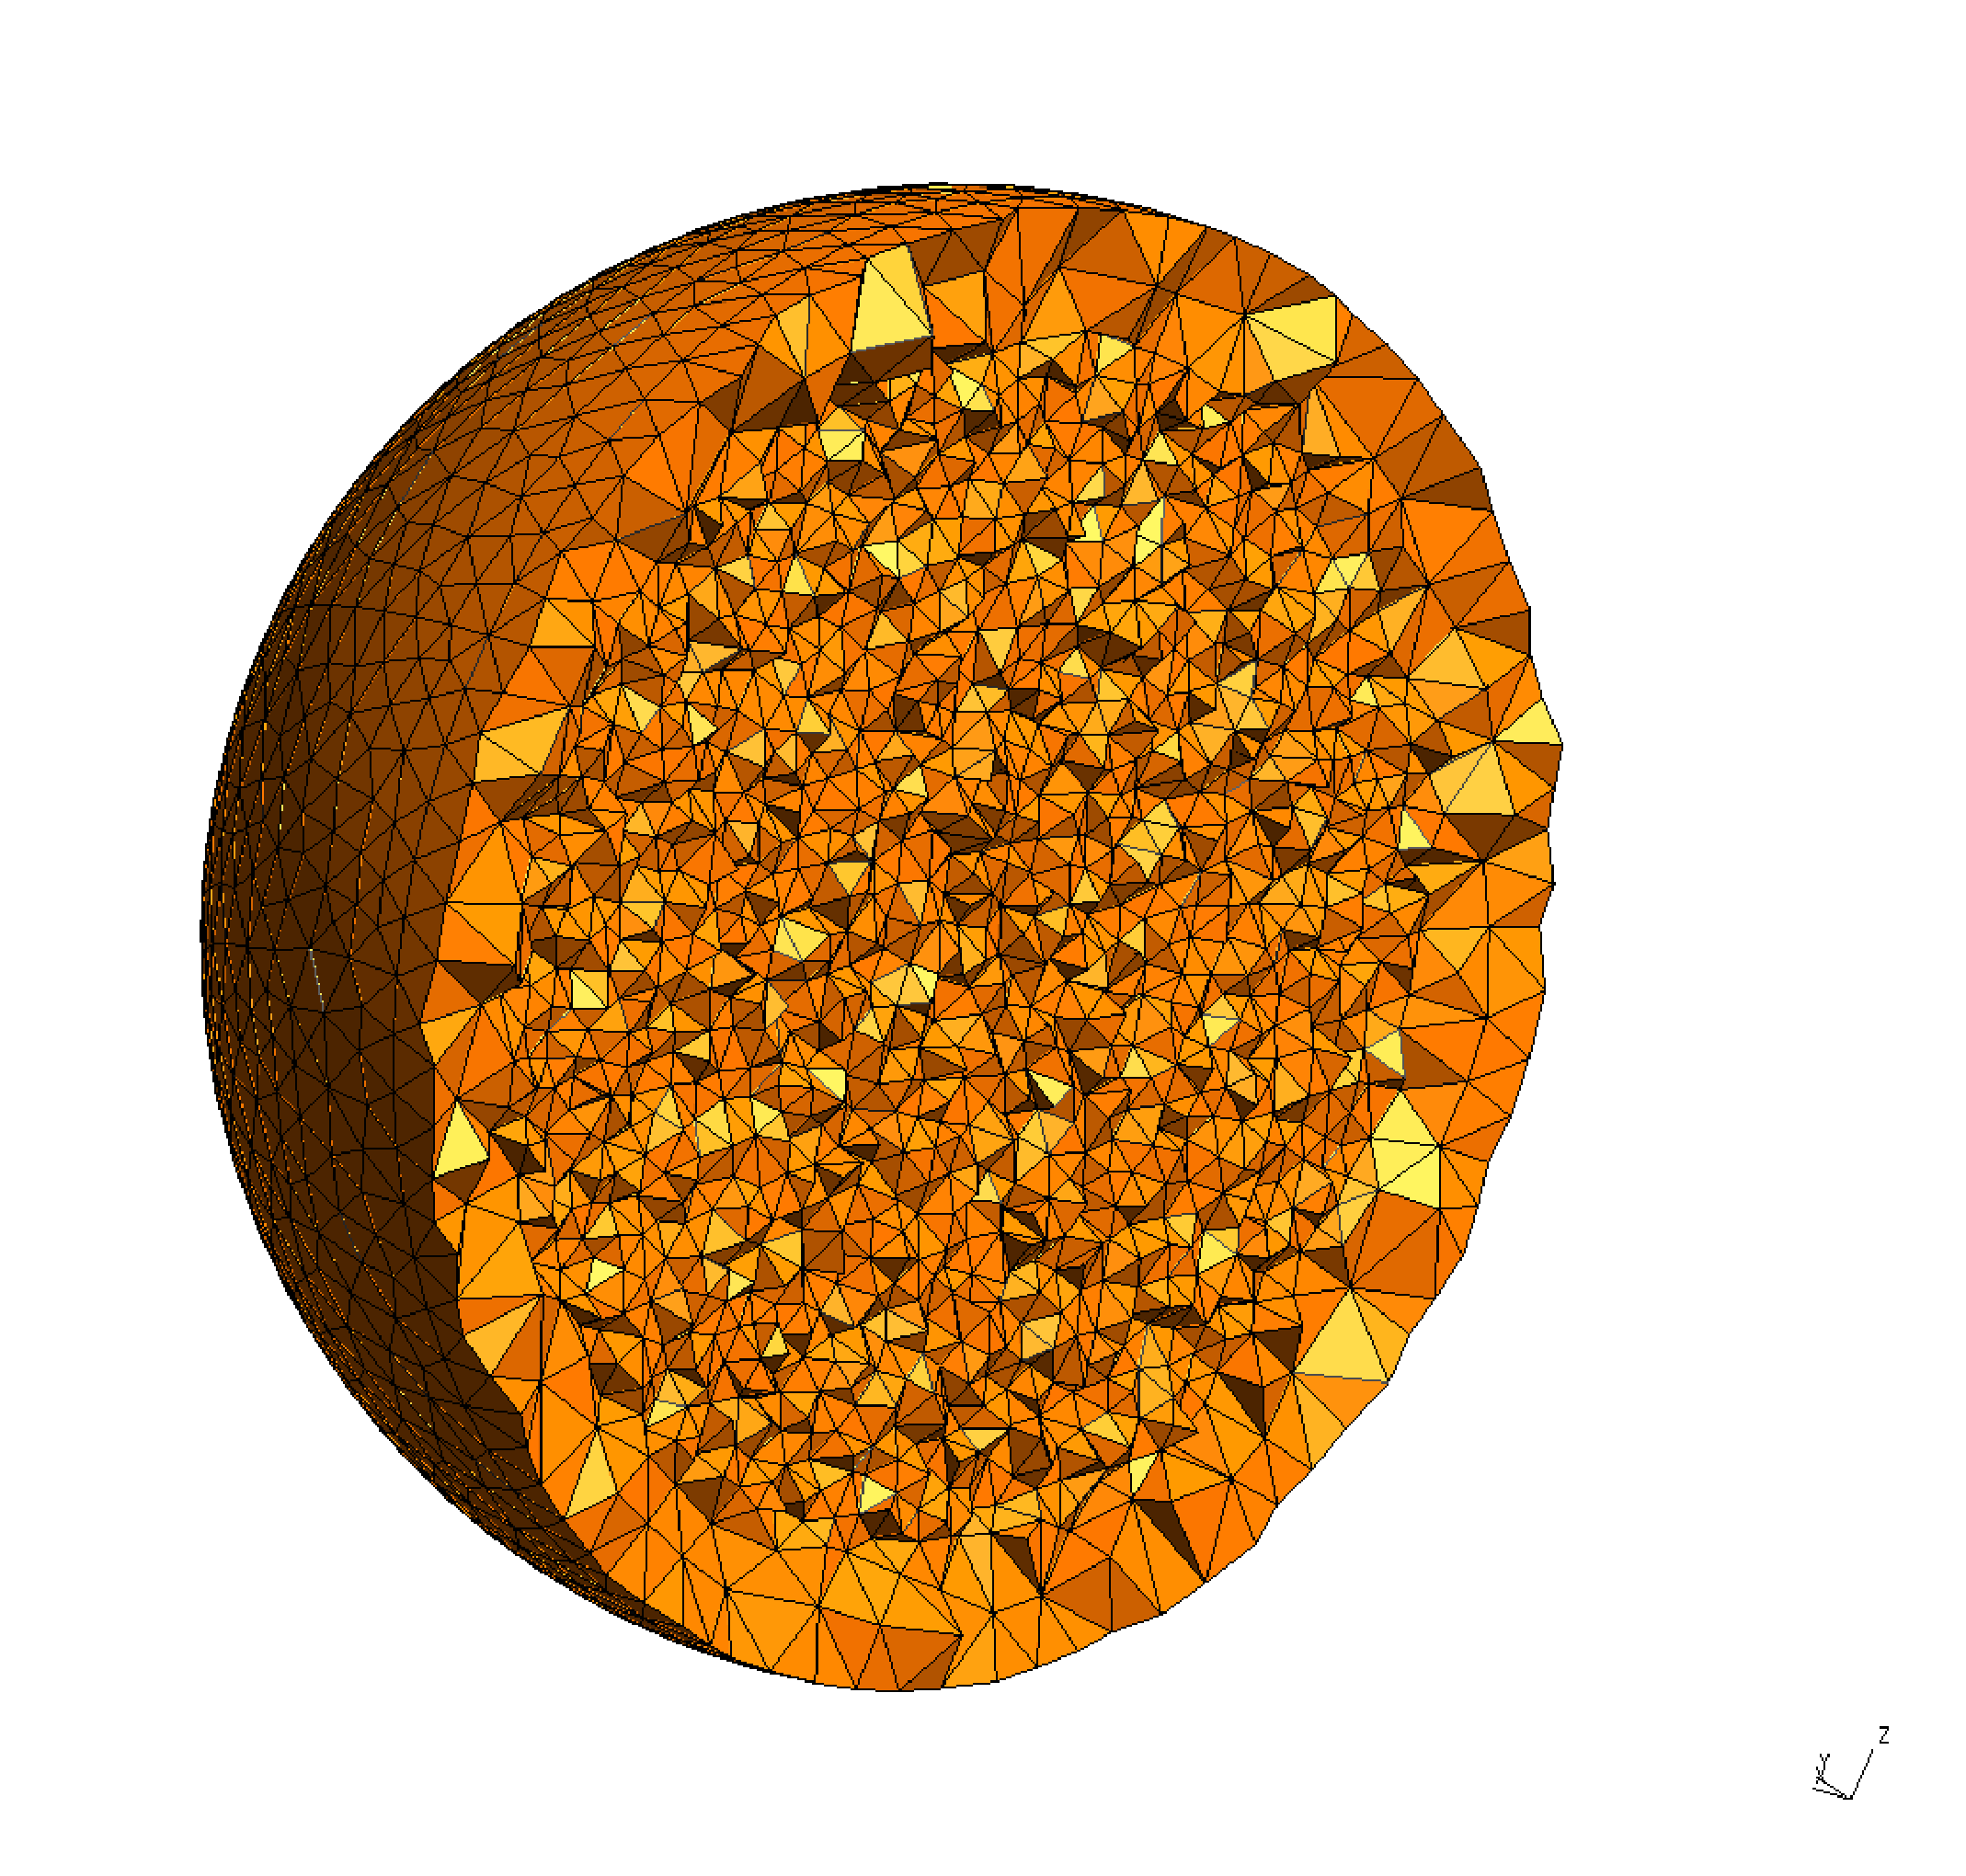
\includegraphics[scale=0.20]{./Pho/Chp4/3d_explosion_coarse_mesh.pdf}
    % \caption{LCD}
  \end{subfigure}%
  ~
  % \begin{subfigure}[b]{0.5\textwidth}
  \begin{subfigure}[b]{0.4\textwidth}
    \centering
    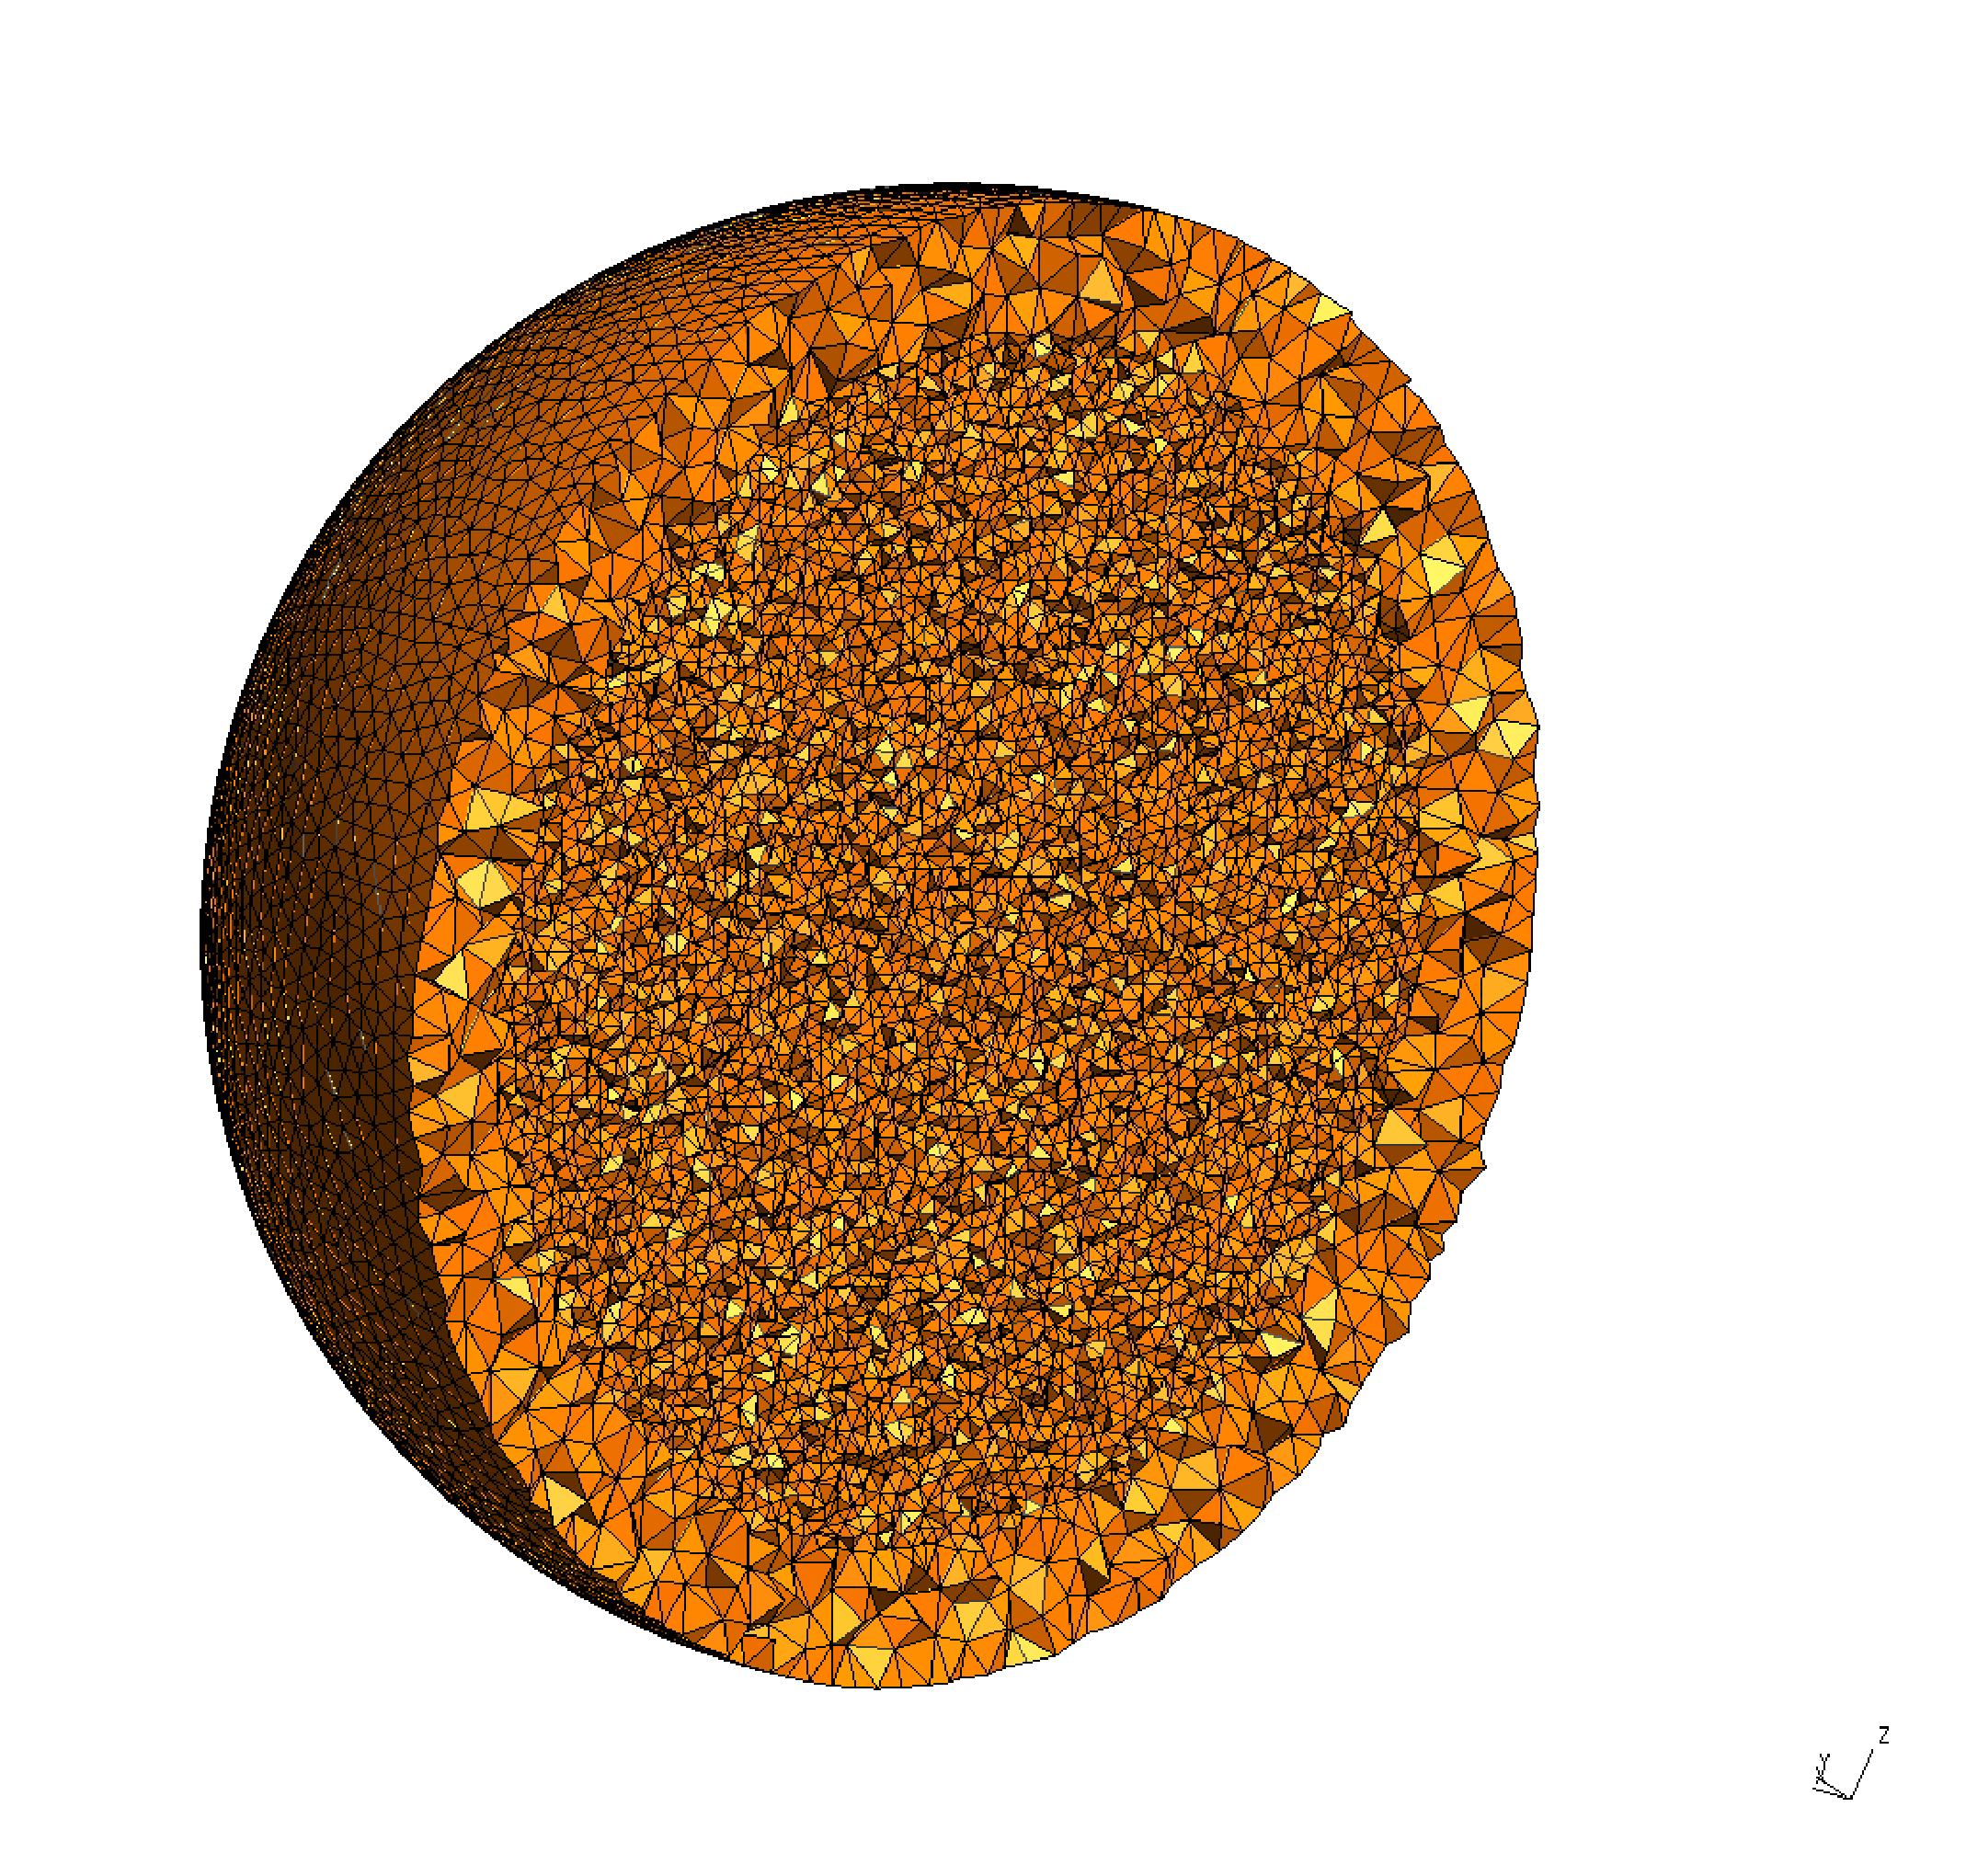
\includegraphics[scale=0.20]{./Pho/Chp4/3d_explosion_fine_mesh.pdf}
    % \caption{Barth}
  \end{subfigure}
  \caption{三维爆炸问题所用四面体计算网格}
  \label{fig:3d-explosion-mesh}
\end{figure}
在计算中我们采用粗细两套计算网格进行对比. 相关的参数如下,
\begin{description}
\item[粗网格] 单元个数: 177379, 单元特征尺寸 (内部区域)
  $\mbox{lc} = 0.04$,
\item[细网格] 单元个数: 1399746, 单元特征尺寸 (内部区域)
  $\mbox{lc} = 0.02$.
\end{description}
两组网格的计算结果对比如
图(\ref{fig:3d-explosion-meshrefine-result}) 所示. 四张图片分别展
示密度、径向速度、压强和内能在径向上的分布. 实线则表示了使用一维
高阶解法器得到的参考解. 另外所有数值解的输出都是在径向
${\bf{n}}_{r} = (1,1,1)$ 上从球心到球面均匀的取 $100$ 个采样点.

从计算结果可以看出, 该求解器可以相对准确的模拟三维爆炸问题, 并且有
效的抑制了间断处的数值震荡. 但是应用了 Barth-Jespersen 限制器
的 MUSCL 重构还是会引入了很大的数值耗散, 使得对间断的解析程度较
差. 另外网格加密会显著提升中心区域解的近似程度, 但是在外围区域精度
提升不明显.

\begin{figure}[htbp]
  \centering
  \includegraphics[scale=1.2]{./Pho/Chp4/3d_explosion_fine_multiplot.pdf}
  \caption{三维爆炸问题计算结果}
  \label{fig:3d-explosion-meshrefine-result}
\end{figure}
\begin{figure}[htbp]
  \centering
  \begin{subfigure}[b]{0.4\textwidth}
    \centering
    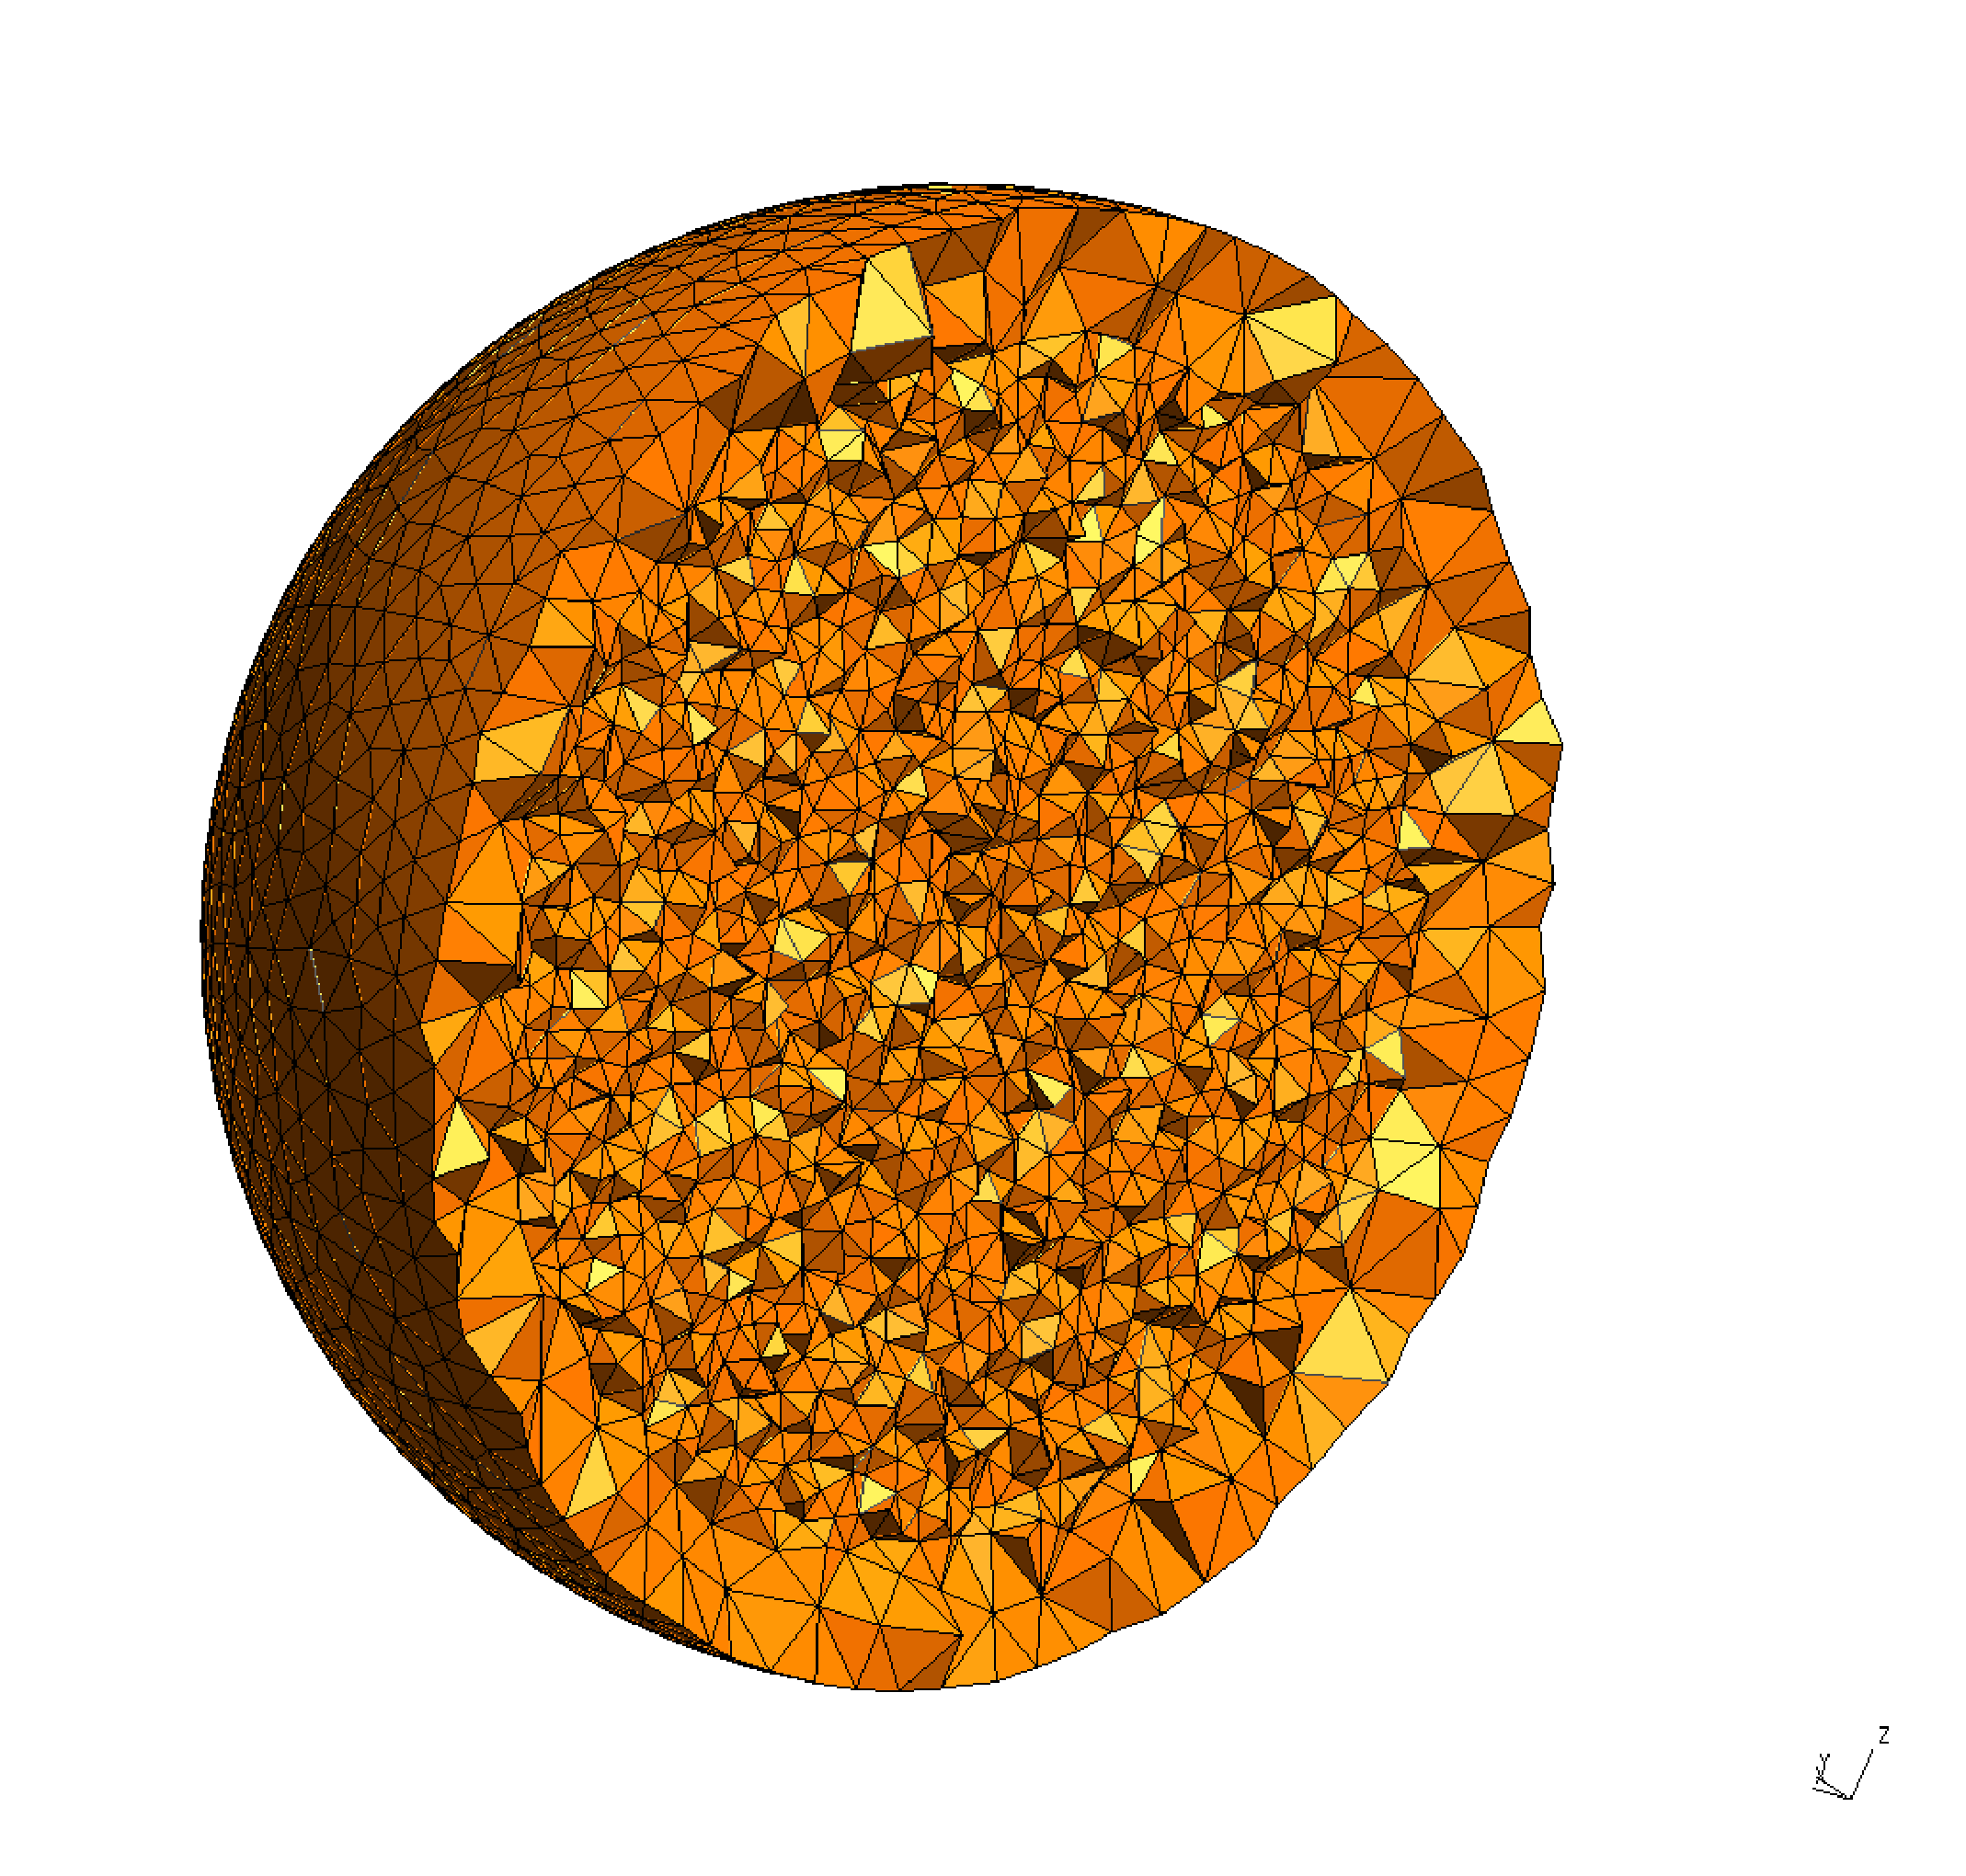
\includegraphics[scale=0.20]{./Pho/Chp4/3d_explosion_coarse_mesh.pdf}
  \end{subfigure}%
  ~
  \begin{subfigure}[b]{0.4\textwidth}
    \centering
    \includegraphics[scale=0.20]{./Pho/Chp4/3d_explosion_adaptive_first_step_mesh.pdf}
  \end{subfigure}
  \caption{初始网格与经自适应之后网格的对比}
  \label{fig:3d-explosion-adaptive-mesh-compare}
\end{figure}
\begin{figure}[htbp]
  \centering
  \includegraphics[scale=1.2]{./Pho/Chp4/3d_explosion_adapt_multiplot.pdf}
  \caption{h-自适应计算结果对比}
  \label{fig:h-adaptive-result-compare}
\end{figure}

基于后验误差估计的自适应策略是提高数值格式精度的有效手段. 在自适应
策略中, 依据后验误差估计对网格进行放粗和加密的方法称为 h-自适应方
法. 我们在三维爆炸问题的数值算例中对 h-自适应方法进行了尝
试. 误差指示子采用如下计算策略,
\begin{equation}
  \label{eq:error-indicator}
  \eta (T_{j}) = h^{3} \min_{k=1,\cdots,4} \left|
    \phi(\bar{\bf{U}}_{j}) - \phi(\bar{\bf{U}}_{j,k}) \right|,
\end{equation}
其中 $\phi(\bar{{\bf{U}}}) = \rho$. 并采用如下的标记策略,
\begin{equation}
  \label{eq:marking-strategy}
  \begin{aligned}
    & M_{r} = \left\{ T_{j}; T_{j}\in \mathcal{T}, ~\eta (T_{j})>
      \beta ~ \max_{T_{j}\in \mathcal{T}} \eta(T_{j})  \right\},
    \quad (\mbox{待加密网格})\\
    & M_{c} = \left\{ T_{j}; T_{j} \in \mathcal{T}, ~\sigma \beta
      \max_{T_{j}\in \mathcal{T}} \eta (T_{j}) \right\}, \quad
    \mbox{待放粗网格}
  \end{aligned}
\end{equation}
其中 $\sigma, \beta$ 为控制加密放粗网格数目的人为参数.

计算初始网格为前面的粗网
格, 图 (\ref{fig:3d-explosion-adaptive-mesh-compare}) 对比了初始网
格与计算过程最初几个时间步之后进行加密的网格. 自适应算法正确识别了
间断位置, 并在内外两个区域的交界处对网格进行了加密处理. 其计算结果
如图 (\ref{fig:h-adaptive-result-compare}) 所示. 该算例在使用h-自
适应策略之后精度方面有所提升, 但是提升幅度十分有限. 其主要原因在
于算例中所采用的后验误差指示子的设计比较简单. 寻找合适的误差指示
子也是该课题的重要后续工作.

\subsection{并行效率}
\label{sec:parallel-efficiency}

并行效率 (Parallel Efficiency) 是衡量一个并行程序对计算资源利用效
率的一个重要指标. 记 $T_{\mbox{serial}}, T_{{\mbox{parallel}}}$ 分
别为同一个算法串行版本和并行版本所需要的计算时间. 假设所使用的处理
器个数为 $p$, 那么并行效率的定义为,
\begin{equation}
  \label{eq:def-parallel-efficiency}
  E = \frac{T_{{\mbox{serial}}}}{p \cdot T_{\mbox{parallel}}}.
\end{equation}
在下面的数值算例中主要考虑两种意义上的并行效率. 第一种情况是保持计
算问题规模不变, 增大进程个数. 在这个意义上测得的并行效率反映了并行
程序的 {\it 强可扩展性}. 而第二种情况是保持计算规模与处理器个数以
同等比例增大的情况下测试其并行效率, 即测试并行程序的 {\it 弱可扩展
  性}. 本节以 (\ref{sec:3d-explosion-test-case}) 节中介绍的三维球对称爆炸
问题对程序的可扩展性进行测试.

\begin{description}

\item[强可扩展性] 首先考虑强可扩展性测试. 测试下面三种情况,
  \begin{itemize}
  \item 粗网格 (单元个数为 177379), 且无自适应加密,
  \item 细网格 (单元个数为 1399746), 且无自适应加密,
  \item 粗网格 (单元个数为 177379), 应用自适应加密.
  \end{itemize}
  依次使用 $8, 32, 64, 128$ 个处理器对问题进行求解, 记录总计算时
  间. 计算数据如
  表 (\ref{tb:strong-parallel-scalabiblity}) 所示. 图
  (\ref{fig:parallel-efficiency-compare}) 则以图像的形式对三种问题
  背景的并行效率进行了对比.
  由计算数据可以看出, 一方面计算问题的规模对并行效率有着显著的影
  响. 例如, 在采用 128 个进程做并行时, 粗网格上的并行效率仅
  为$67\%$, 而细网格对应的并行效率则可以达到 $89\%$. 另一方面, 使用
  自适应策略之后的并行效率要低于未做自适应的情况. 造成这种情况的原
  因, 首先是因为自适应算法会造成而外的通讯时间. 另外网格加密也会使
  加密后的计算规模要大于初始计算规模, 从而使得测得的并行效率偏低.
  \begin{center}
    \scriptsize
    \begin{table}
      
\begin{center}
\begin{tabular}{r|rr|rr|rr}
% \hline
   & \multicolumn{2}{c}{自适应加密(粗网格)} & \multicolumn{2}{c}{
     无自适应加密(粗网格)} &  \multicolumn{2}{c}{无自适应加密(细网格)}      \\
\hline
 进程数  &        计算时间 (m)  &  并行效率  &              计算
 时间 (m)  &  并行效率  &              计算时间 (m)  &  并行效率  \\
\hline
      8  &             2308.60  &         1  &                692.57  &         1  &              19666.39  &         1  \\
     32  &              642.43  &    0.8984  &                184.80  &    0.9369  &               4971.30  &    0.9890  \\
     64  &              416.27  &    0.6932  &                100.64  &    0.8602  &               2540.81  &    0.9675  \\
    128  &              287.47  &    0.5019  &                 63.09  &    0.6861  &               1386.51  &    0.8865  \\
\hline
\end{tabular}
\end{center}

      \caption{强可扩展性测试结果}
      \label{tb:strong-parallel-scalabiblity}
    \end{table}
  \end{center}
  % \begin{figure}[htbp]
  \begin{figure}
    \centering
    \includegraphics[scale=1.0]{./Pho/Chp4/parallel_efficiency.pdf}
    \caption{三种问题背景的强可扩展性对比}
    \label{fig:parallel-efficiency-compare}
  \end{figure}
\item[弱可扩展性] 表 (\ref{tb:strong-parallel-scalabiblity}) 最后
  两组数据的对比可以看出. 如果固定进程个数, 并行效率会随着问题规模
  的增大而提高. 可见问题规模会显著影响并行效率. 在下面的测试算例
  中, 在增大问题规模的同时控制单个进程的平均载荷固定不变, 即保持单
  元数与进程数之比 $\mbox{NElem}/\mbox{NProc}$ 近似定常.  计算结果
  如表 (\ref{tb:weak-parallel-scalabiblity}) 所示. 千核并行时仍可
  以保持较好的可扩展性.
  \begin{center}
    \scriptsize
    \begin{table}
              \begin{tabular}{rrrrrr}
          单元特征尺寸  &  单元个数  &  处理器个数  &  单元数/处理器个数  &  timestep / s  &  弱可扩展性  \\
          \hline
          0.16300  &     21808  &           2  &         10904.0000  &        5.1974  &           1  \\
          0.08045  &    174737  &          16  &         10921.0630  &        4.7773  &      0.9192  \\
          0.04000  &   1399746  &         128  &         10935.5160  &        3.9986  &      0.7693  \\
          0.02000  &  11181578  &        1024  &
          10919.5100  &        2.5627  &      0.4931\\
          \hline
        \end{tabular}

      \caption{弱并行可扩展性}
      \label{tb:weak-parallel-scalabiblity}
    \end{table}
  \end{center}
  % , 时间推进速率为两个进程情形时间推进
  % 速度的 $50\%$ 左右.
\end{description}
